\documentclass[11pt,a4paper]{article}
\usepackage[margin=2.5cm]{geometry}
\usepackage[T1]{fontenc}
\usepackage{lmodern}
\usepackage{amsmath}
\usepackage{graphicx}
\usepackage{xcolor}
\usepackage{booktabs}
\usepackage{hyperref}
\usepackage{tikz}
\definecolor{TSLRed}{RGB}{199,25,24}
\hypersetup{colorlinks=true,linkcolor=TSLRed,citecolor=TSLRed,urlcolor=TSLRed}
\title{\textcolor{TSLRed}{Projected Column Density of the Eta Carinae Homunculus}\\\large First-stage infinitesimally thin-shell model}
\author{Reproducible Julia implementation}
\date{\today}
\begin{document}
\maketitle

\begin{abstract}
This report documents a first-stage map of the mass column density seen by an observer through the Homunculus of Eta Carinae. The model treats the lobes as an axisymmetric, ballistic, infinitesimally thin surface, uses the supplied latitude-dependent mass distribution and velocity curve, normalizes the shell mass to $1\,M_\odot$, and adds all shell intersections along every sightline. The map is therefore a geometric baseline, rather than a fit to an image.
\end{abstract}

\section{Observational geometry}
The calculation uses the outer molecular shell geometry of Smith \cite{smith2006}: the polar symmetry axis is inclined by $41.0^\circ\pm0.5^\circ$ from the line of sight. This convention is stated explicitly because it is equivalently $49.0^\circ$ from the sky plane. The projected polar axis has PA $310^\circ$ for the NW/red lobe (or $130^\circ$ for the SE/blue lobe); PA only rotates an axisymmetric model on the sky, so the generated image places the projected axis vertically. The ballistic age uses the HST proper-motion ejection epoch $1847.1\pm0.8$ \cite{smith2017}, evaluated at image epoch 2000.0, giving 152.9 yr.

\section{Thin-shell formulation}
Let $f(\lambda)$ be the supplied $d\tilde m/d\Omega$, where the input angle $\lambda$ is latitude from the equator. It is evaluated with a shape-preserving cubic interpolant and mirrored about the equator, then normalized so that
\begin{equation}
 dM = M_\mathrm{shell}\,\frac{f(\lambda)}{\int f\,d\Omega}\,d\Omega,
 \qquad M_\mathrm{shell}=1\,M_\odot.
\end{equation}
The input velocity curve sets the surface radius through homologous expansion,
\begin{equation}
 r(\lambda)=v(\lambda)\,[2000.0-1847.1].
\end{equation}
For a radial surface element, $dA/d\Omega=r^2/|\hat{r}\cdot\hat n|$. Its surface density and projected contribution are therefore
\begin{equation}
 \Sigma_\mathrm{surf}=\frac{dM}{d\Omega}\frac{|\hat r\cdot\hat n|}{r^2},
 \qquad
 \Sigma_\mathrm{LOS}=\sum_k\frac{\Sigma_{\mathrm{surf},k}}{|\hat n_k\cdot\hat\ell|}.
\end{equation}
This is the unambiguous surface-projection form of the handwritten/OCR equation. The summation is implemented by rasterizing all surface triangles and adding, rather than depth-clipping, their contributions. It includes front and rear shell crossings; the same approach supports additional crossings once a non-convex surface is introduced.

\section{Implementation and result}
\texttt{thin\_shell\_column\_density.jl} uses only Julia standard libraries. It produces a false-colour PPM/PNG map, a numeric CSV grid in g cm$^{-2}$, and metadata. The numerical map has no opacity law: it is material column density.

\begin{figure}[ht]
\centering
\begin{minipage}{0.65\linewidth}
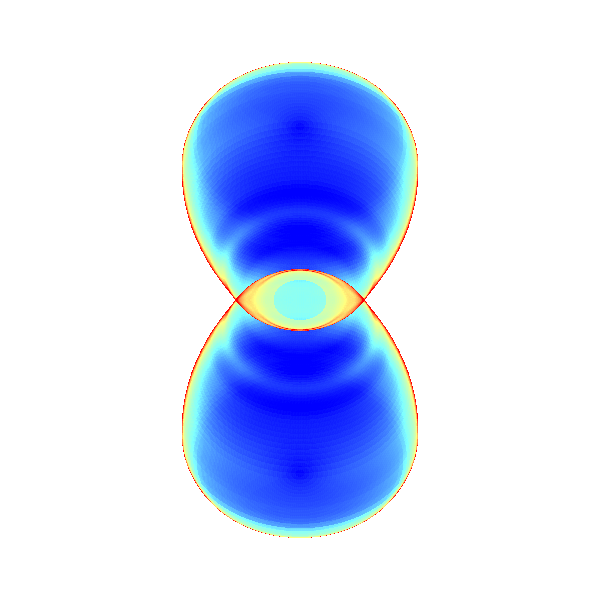
\includegraphics[width=\linewidth]{output/thin_shell_column_density.png}
\end{minipage}\hfill
\begin{minipage}{0.27\linewidth}\centering
\textbf{$\log_{10}\Sigma_{\rm LOS}$}\\[-0.4em]
\textbf{(g cm$^{-2}$)}\\[0.4em]
\begin{minipage}[c][5cm][c]{0.30\linewidth}\raggedleft
\textbf{-1.005}\vfill
\textbf{-1.5}\vfill
\textbf{-2.0}\vfill
\textbf{-2.130}
\end{minipage}%
\begin{minipage}[c][5cm][c]{0.42\linewidth}

\includegraphics[width=\linewidth,height=5cm]{output/thin_shell_column_density_colourbar.png}
\end{minipage}
\end{minipage}
\caption{Projected total gas column density for an infinitesimally thin, $1\,M_\odot$ shell. The colour scale is logarithmic and spans the 2nd to 99.5th percentiles of non-zero map values: $-2.130 \leq \log_{10}(\Sigma_{\rm LOS}/\mathrm{g\,cm^{-2}}) \leq -1.005$. White is outside the projected surface. Bright rims arise from the $1/|\hat n\cdot\hat\ell|$ projection factor.}
\end{figure}

\section{Finite-duration ejection}
The thin-shell result is extended by treating the measured 1847.1 epoch as the midpoint of a constant-mass-loss interval of $\Delta T=20$ yr. The same total mass, $1\,M_\odot$, is divided equally among 101 launch-time layers. A layer launched at offset $\delta t$ has present-day radius $r(\lambda)=v(\lambda)(t_{\rm obs}-1847.1-\delta t)$, and the final map is the sum of its projected columns. This is a numerical quadrature of a radial volume shell: at latitude $\lambda$ its width is $\Delta r(\lambda)=v(\lambda)\Delta T$. It assumes the angular mass distribution and speed were constant throughout the 20 years.

\begin{figure}[ht]
\centering
\begin{minipage}{0.65\linewidth}
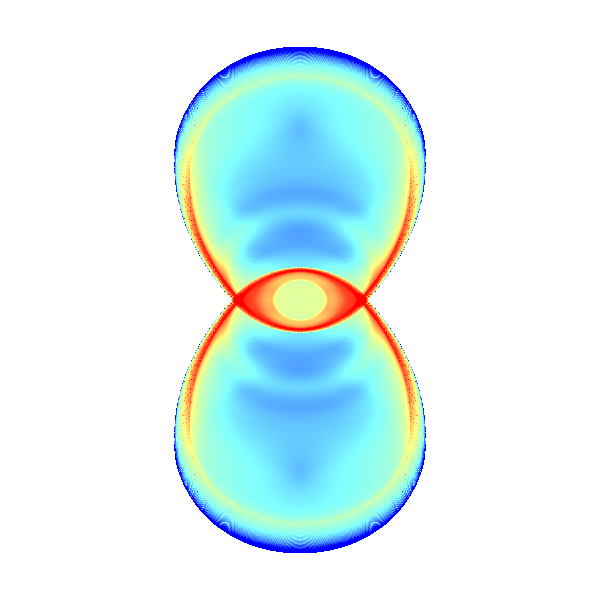
\includegraphics[width=\linewidth]{output/finite_duration_column_density.png}
\end{minipage}\hfill
\begin{minipage}{0.27\linewidth}\centering
\textbf{$\log_{10}\Sigma_{\rm LOS}$}\\[-0.4em]
\textbf{(g cm$^{-2}$)}\\[0.4em]
\begin{minipage}[c][5cm][c]{0.30\linewidth}\raggedleft
\textbf{-1.267}\vfill
\textbf{-1.5}\vfill
\textbf{-2.0}\vfill
\textbf{-2.375}
\end{minipage}%
\begin{minipage}[c][5cm][c]{0.42\linewidth}

\includegraphics[width=\linewidth,height=5cm]{output/finite_duration_column_density_colourbar.png}
\end{minipage}
\end{minipage}
\caption{Finite-duration ($\Delta T=20$ yr) ejection model. The logarithmic scale spans the 2nd to 99.5th percentiles of non-zero pixels. Relative to the infinitesimal shell, the limb contribution is spread over the radial width of the flow rather than concentrated in a single surface.}
\end{figure}

\section{Observer-facing shell only}
For the finite-duration shell, the map can be restricted to material facing the observer. Each surface element is assigned an outward unit normal $\hat n$; it contributes only when $\hat n\cdot\hat\ell>0$, where $\hat\ell$ points from the nebula to the observer. This excludes the rear shell crossing. For an oblique ray that crosses the outer boundary twice but does not reach the inner boundary, the two outer crossings have opposite normal orientations. Retaining only the observer-facing one therefore gives one half of their combined column density, as required.

\begin{figure}[ht]
\centering
\begin{minipage}{0.65\linewidth}
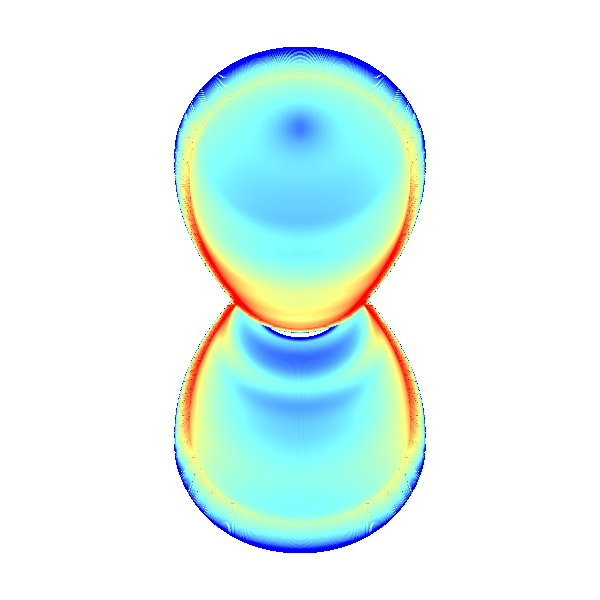
\includegraphics[width=\linewidth]{output/near_side_finite_duration_column_density.png}
\end{minipage}\hfill
\begin{minipage}{0.27\linewidth}\centering
\textbf{$\log_{10}\Sigma_{\rm LOS}$}\\[-0.4em]
\textbf{(g cm$^{-2}$)}\\[0.4em]
\begin{minipage}[c][5cm][c]{0.30\linewidth}\raggedleft
\textbf{-1.592}\vfill
\textbf{-2.0}\vfill
\textbf{-2.5}\vfill
\textbf{-2.708}
\end{minipage}%
\begin{minipage}[c][5cm][c]{0.42\linewidth}

\includegraphics[width=\linewidth,height=5cm]{output/near_side_finite_duration_colourbar.png}
\end{minipage}
\end{minipage}
\caption{Observer-facing component of the $\Delta T=20$ yr model with a $10^\circ$ equatorial cutoff applied only to this near-side selection. The all-crossing maps retain the complete supplied angular distribution. The scale is logarithmic and spans the 2nd to 99.5th percentiles of non-zero pixels: $-2.708 \leq \log_{10}(\Sigma_{\rm LOS}/\mathrm{g\,cm^{-2}}) \leq -1.592$.}
\end{figure}

\clearpage

\section{STL finite-width model}
The analysis was repeated using the supplied binary STL surface, which contains 17,101 triangles. Its longest dimension is the native $z$ direction, adopted as the intrinsic polar axis. The mesh is scaled uniformly so that its largest polar radius equals the Smith-based pole at epoch 2000,
\begin{equation}
 R_{\rm pole}=v(90^\circ)(2000.0-1847.1)=3.1215\times10^{17}\ {\rm cm}=20{,}866\ {\rm AU}.
\end{equation}
This gives $8.1915\times10^{16}$ cm per native STL unit. The same $41^\circ$ axis-to-line-of-sight inclination is then applied.

The smoothed Smith mass-per-solid-angle function is evaluated at each triangle's centroid latitude. For triangle $j$, its angular weight is
\begin{equation}
 w_j=f(\lambda_j)\,\Delta\Omega_j,
 \qquad
 \Delta\Omega_j\simeq A_j\frac{|\hat r_j\cdot\hat n_j|}{r_j^2},
\end{equation}
and triangle masses are normalized as $m_j=M_\odot w_j/\sum_k w_k$. A 20-year ejection width is included using 101 homologously scaled launch-time layers, each carrying $1/101$ of every triangle's mass. All projected intersections are added, so this figure is the total column density rather than the observer-facing-only variant.

\begin{figure}[ht]
\centering
\begin{minipage}{0.65\linewidth}
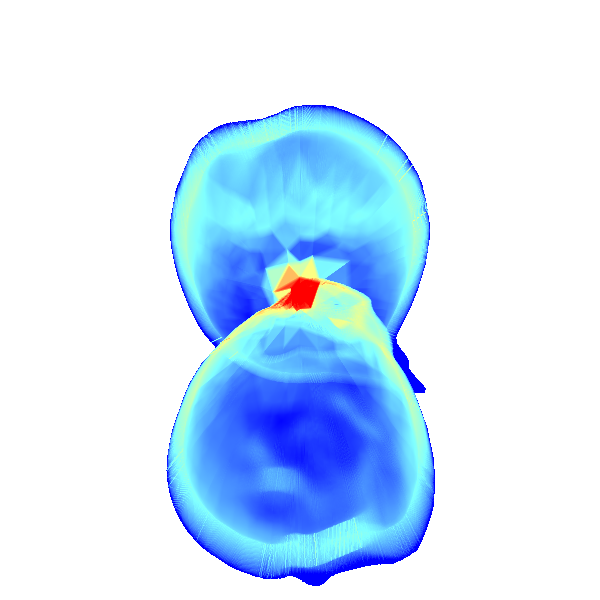
\includegraphics[width=\linewidth]{output/stl_finite_duration_column_density.png}
\end{minipage}\hfill
\begin{minipage}{0.27\linewidth}\centering
\textbf{$\log_{10}\Sigma_{\rm LOS}$}\\[-0.4em]
\textbf{(g cm$^{-2}$)}\\[0.4em]
\begin{minipage}[c][5cm][c]{0.30\linewidth}\raggedleft
\textbf{-0.620}\vfill
\textbf{-1.0}\vfill
\textbf{-1.5}\vfill
\textbf{-2.0}\vfill
\textbf{-2.5}\vfill
\textbf{-2.800}
\end{minipage}%
\begin{minipage}[c][5cm][c]{0.42\linewidth}

\includegraphics[width=\linewidth,height=5cm]{output/stl_finite_duration_colourbar.png}
\end{minipage}
\end{minipage}
\caption{Total projected column density of the scaled STL Homunculus for $M=1\,M_\odot$ and $\Delta T=20$ yr. The logarithmic display spans the 2nd to 99.5th percentiles of non-zero pixels. Non-axisymmetric structure comes directly from the STL mesh.}
\end{figure}

The rasterization is mass-conservative: each triangle's mass is divided among the sky pixels covered by its projection. Integrating the resulting map over pixel area recovers $1.00000000\,M_\odot$. The numerical map is written in g cm$^{-2}$, with a separate AU coordinate vector defining both sky axes.

\clearpage

\section{Spectral-aperture optical depths}
Figure~4 of Smith et al. (2003) defines the locations used for the spatially resolved spectra, while Figure~2d provides the corresponding cool-dust $18\,\mu$m emission optical-depth contours. The overlay below registers the apertures by matching the outer Homunculus extent, rather than forcing the central-star positions to coincide. This is the preferred transform for the extended cool-dust shell. Solid boxes labelled 1 and 2 are the representative polar-lobe spectral apertures; the other labelled boxes sample the core and inner structure.

\begin{figure}[ht]
\centering
\begin{tikzpicture}
\node[inner sep=0] (image) at (0,0) {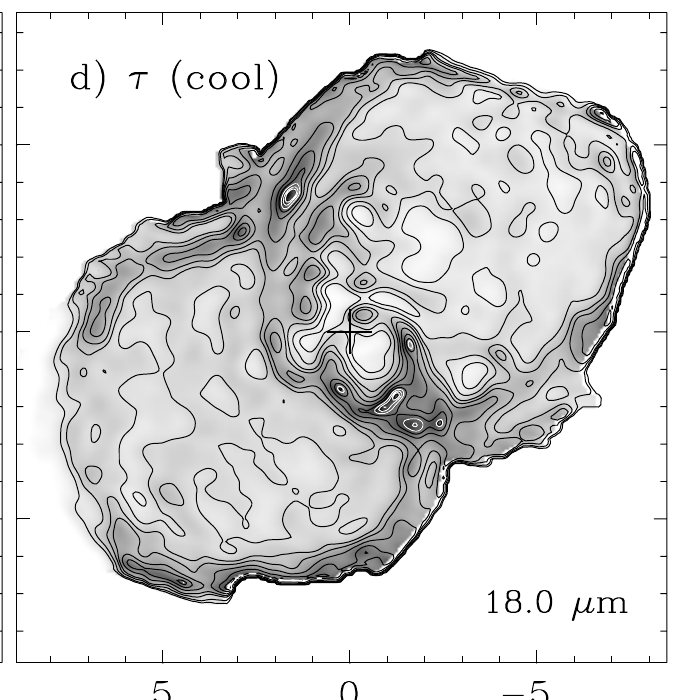
\includegraphics[width=0.76\linewidth]{output/smith_2003_fig2d.png}};
\begin{scope}[x={(image.south east)},y={(image.north west)}]
\tikzset{aperture/.style={draw=TSLRed,line width=0.8pt,fill=none}}
\draw[aperture] (0.49,0.49) rectangle (0.56,0.56) node[above right,black,font=\scriptsize] {core};
\draw[aperture] (0.42,0.54) rectangle (0.48,0.61) node[above left,black,font=\scriptsize] {NE};
\draw[aperture] (0.46,0.45) rectangle (0.52,0.52) node[below left,black,font=\scriptsize] {SE};
\draw[aperture] (0.48,0.40) rectangle (0.54,0.47) node[below left,black,font=\scriptsize] {S};
\draw[aperture] (0.54,0.39) rectangle (0.61,0.45) node[below right,black,font=\scriptsize] {SW};
\draw[aperture] (0.38,0.64) rectangle (0.43,0.70) node[above left,black,font=\scriptsize] {NE2};
\draw[aperture] (0.19,0.58) rectangle (0.25,0.65) node[above left,black,font=\scriptsize] {1};
\draw[aperture] (0.20,0.33) rectangle (0.30,0.44) node[below left,black,font=\scriptsize] {2};
\end{scope}
\end{tikzpicture}
\caption{Smith et al. (2003) Figure~2d ($\tau_{18\,\mu\mathrm{m}}$ of cool dust) with Figure~4 spectral apertures registered by matching the outer Homunculus extent. The source image is reproduced from the local copy of Smith et al. (2003); red annotations are added here.}
\end{figure}

The published contours are $\tau_{18}=0.05, 0.1, 0.2, 0.3, 0.5, 0.8, 1.1, 1.4, 1.8,$ and $2.2$. Reading the outer-extent-registered apertures against those contours gives the following preliminary values. They are intended for selecting regions for spectral fitting, with an uncertainty of at least one contour interval from the figure registration and contour-only digitisation.

\begin{table}[ht]
\centering
\caption{Preliminary cool-dust $18\,\mu$m optical-depth estimates from Smith et al. (2003) Figure~2d.}
\begin{tabular}{lll}
\toprule
Spectral region & $\tau_{18\,\mu\mathrm{m}}$ estimate & Interpretation \\
\midrule
core & $1.1$--$2.2$ & optically thick inner cool-dust structure \\
NE, SE & $0.5$--$1.1$ & inner lobe/core transition \\
S, SW & $0.3$--$0.8$ & inner southern structure \\
NE2 & $0.2$--$0.5$ & overlap/outer-inner transition \\
1 (lobe edge) & $0.5$--$1.1$ & limb-brightened cool shell \\
2 (lobe middle) & $0.1$--$0.3$ & interior lobe sightline \\
\bottomrule
\end{tabular}
\end{table}

For comparison to the mass-column maps, a dust model supplies $\tau_{18}=\kappa_{18}\Sigma_{\rm LOS}$, where $\kappa_{18}$ is the mass absorption coefficient for the chosen gas-plus-dust convention. The contour estimates above can therefore constrain an effective $\kappa_{18}$, or test whether a single opacity is adequate, once the aperture registration is transferred to the model coordinate system.

\section{Limitations and next stage}
The supplied functions are evaluated with a shape-preserving piecewise-cubic Hermite interpolant, rather than linear segments, removing artificial slope discontinuities while preserving each tabulated value and avoiding cubic overshoot. The surface remains axisymmetric and exactly homologous; it mirrors the input curves between hemispheres. It omits radiative transfer, dust opacity, clumps, equatorial material, temporal changes in the mass/angular or velocity distributions, and documented modest non-homologous deviations \cite{steffen2014}. A next refinement can replace the launch-time-layer quadrature with direct ray integration through a specified continuous density law.

\begin{thebibliography}{9}
\bibitem{smith2006} Smith, N. 2006, \emph{ApJ}, 644, 1151. \href{https://doi.org/10.1086/503766}{doi:10.1086/503766}.
\bibitem{smith2017} Smith, N. 2017, \emph{MNRAS}, 471, 4465. \href{https://doi.org/10.1093/mnras/stx1868}{doi:10.1093/mnras/stx1868}.
\bibitem{steffen2014} Steffen, W. et al. 2014, \emph{MNRAS}, 442, 3316. \href{https://doi.org/10.1093/mnras/stu1088}{doi:10.1093/mnras/stu1088}.
\end{thebibliography}
\end{document}
